% TEXINPUTS=.:$HOME/git/bvtex: latexmk  -pdf <main>.tex
\documentclass[xcolor=dvipsnames]{beamer}

\input{defaults}
\input{beamer/preamble}

\setbeamertemplate{navigation symbols}{}
% \setbeamertemplate{background}[grid][step=1cm]

\usepackage{siunitx}
\usepackage{xmpmulti}
\usepackage[export]{adjustbox}
\usepackage{ulem}
\usepackage[outline]{contour}
\usepackage{pdfpages}
\usepackage{tikz}
\usetikzlibrary{shapes.geometric, arrows}
\usetikzlibrary{positioning}

\definecolor{bvtitlecolor}{rgb}{0.98, 0.92, 0.84}
\definecolor{bvoutline}{rgb}{0.1, 0.1, 0.1}

\renewcommand{\bvtitleauthor}{Brett Viren\\\footnotesize(for W-C team)}
\renewcommand{\bvtit}{WCTV}
\renewcommand{\bvtitle}{\LARGE Wire-Cell Validation\\``Systems''}
\renewcommand{\bvevent}{$\mu$B Reco\\2017 Dec 12}
\renewcommand{\bvbeamerbackground}{}

\begin{document}
\input{beamer/title.tex}
\input{beamer/toc.tex}

\section{Background}

\begin{frame}
  \frametitle{Wire-Cell Feature Overview}
  \textbf{Toolkit}:
  \begin{itemize}\footnotesize
  \item \textbf{noise filter} coherent, harmonic, PMT, etc.  $\sim\mu$B-specific.
  \item \textbf{signal processing} broad+fine 2D deconvolution and ROI-finder.
  \item \textbf{signal simulation} drift physics, broad+fine 2D field/elec responses, ADC.
  \item \textbf{noise simulation} spectral sampling with MicroBooNE empiric noise model.
  \end{itemize}
  \scriptsize Toolkit functionality available via provided
  \texttt{wire-cell} command line program, through user-application or, to
  some extent, via \textit{art}/LArSoft integration (next slide).

  \vfill

  \normalsize
  \textbf{Prototype}:
  \begin{itemize}\footnotesize
  \item Incubator for code that eventually goes into the toolkit.
  \item Now incubating: \textbf{3D imaging}, \textbf{clustering} and \textbf{pattern recognition}.
  \end{itemize}
  \scriptsize Prototype functionality available via its integration test programs.

  \vfill

  \begin{center}\tiny
    (various software design, development and user technical features omitted here)
  \end{center}

\end{frame}

\begin{frame}
  \frametitle{\textbf{W}ire-\textbf{C}ell / \textbf{L}Ar\textbf{S}oft Integration}
  ``\textbf{WC/LS}''
  \begin{itemize}\footnotesize
  \item Design overview
    \begin{itemize}\scriptsize
    \item call WCT code on each event from inside \textit{art} module via a \textit{art} tool.
    \item formalize WC $\leftrightarrow$ LS data product conversion
    \item job aggregation is fully dynamic (via FHiCL + WC config langs)
    \end{itemize}
  \item Single \texttt{WireCellToolkit\_module} and \texttt{WCLS\_tool} provided.
    \begin{itemize}\scriptsize
    \item Covers most/all use cases, but tool can be used from user modules.
    \end{itemize}
  \item All integration code in LArSoft as \texttt{larwirecell} package.
    \begin{itemize}\scriptsize
    \item A \texttt{wirecell} UPS product build from WCT releases.
    \item All ``heavy lifting'' code in WCT shared libraries.
    \end{itemize}
  \end{itemize}
  Current status and near term:
  \begin{itemize}\footnotesize
  \item[$\times$] Obsolete: old style NF-only module only in MCC 8.x branch.
  \item[$\checkmark$] Done: Noise Filter + Signal Processing targeting MicroBooNE.
  \item[$\to$] Next: Simulation, helped immensely by LArG4 reorg effort.
  \end{itemize}
\end{frame}

\section{Prototype Validation}

\begin{frame}
  \frametitle{Wire-Cell Prototype Validation}
  \begin{itemize}\footnotesize
  \item Initial concepts are developed in the WC \textbf{Prototype} code base.
  \item Conceptual/algorithm validation procedures might be described
    as intensive, data driven and not reproducible (in a CI sense).
  \item A number of \texttt{main()} programs provide both integration
    level testing as well as main applications for initial processing and analysis.
    \begin{itemize}\scriptsize
    \item Test code tends to be somewhat monolithic but with much
      functionality sequestered to the WCP libraries.
    \end{itemize}
  \item [$\to$] We treat results from the prototype as the benchmark
    for what WCT code must reproduce.
  \end{itemize}
\end{frame}

\section{Toolkit and WC/LS Integration Validation}

\begin{frame}
  \frametitle{Wire-Cell Toolkit Validation ``System''\footnote{Scare quotes because many improvements really should be made.}}
  Design: validation suite runs as a \textbf{build system} using \href{https://waf.io/}{WAF}.
    \begin{itemize}\footnotesize
    \item[+] Failures halt the ``build'' and can not be denied.
    \item[+] Test successes need not be rerun after dealing with failures.
    \item[+] Runs various tests, some which depend on others.
    \item[+] Runs tests in parallel to the extent possible given dependencies.
    \item[+] Generates JSON summaries and templated (Jinja2) web pages.
    \item[+] Results: logs, plots, \textbf{diffs}, job errors.
    \item[+] Some hist diffs done automatically, lead to ``build'' failure.
    \item[-] Relies on a few GB of MicroBooNE data files.
    \item[-] Not directly conducive to integrating into ``real'' CI system.
    \item[-] Waf's \texttt{wscript} is powerful but not for everyone.
    \end{itemize}
    
\end{frame}

\begin{frame}[fragile]
  \frametitle{Do a validation build}

  \begin{verbatim}
$ source setup_wcls_environment_is_exercise_for_user
$ ./waf configure  \
      --prefix=$HOME/public_html/wctv \
      --wct-build=/path/to/wct/build \
      --wct-data=/path/to/data/validation
$ ./waf
$ firefox $HOME/public_html/wctv/html
\end{verbatim}

    \begin{center}\footnotesize
      \href{http://www.phy.bnl.gov/~bviren/tmp/wcls/validation/html/}{Click to see results in all their stunning lack of CSS glory}      

      \vfill

      and, here is the code repo:

      \url{https://github.com/WireCell/wire-cell-validate}    
    \end{center}
\end{frame}

\begin{frame}
  \frametitle{Current validation contents}
  \begin{itemize}\footnotesize
  \item Idea is to add a new \texttt{subdir/wscript} file for each test scope.
  \item So far only scope is: NF+SP as WCT vs WC/LS
  \item Run same WCT code as pure \texttt{wire-cell} and \texttt{art} jobs.
  \item Form histograms and event displays for each.
    \begin{itemize}\scriptsize
    \item[$\sim$] (uses Numpy/Matplotlib but ROOT could also be used)
    \end{itemize}
  \item ``Diffs'' between corresponding WCT and WC/LS results.
  \item Produce reduced and full resolution event displays.
  \item Also produce summary/profile hists.
  \item Look for any non-zero content in subtracted hists/displays.
  \item \texttt{foreach} file, \texttt{foreach} event in file, \texttt{foreach} tier.
  \item Processing ``tiers'':
    \begin{itemize}\scriptsize
    \item[$\to$] original ADC, NF'ed ``raw'', ``wiener'' and ``gauss'' filtered signals, 
    \end{itemize}
  \end{itemize}
\end{frame}

\begin{frame}[fragile]
  \frametitle{Original ADC}
  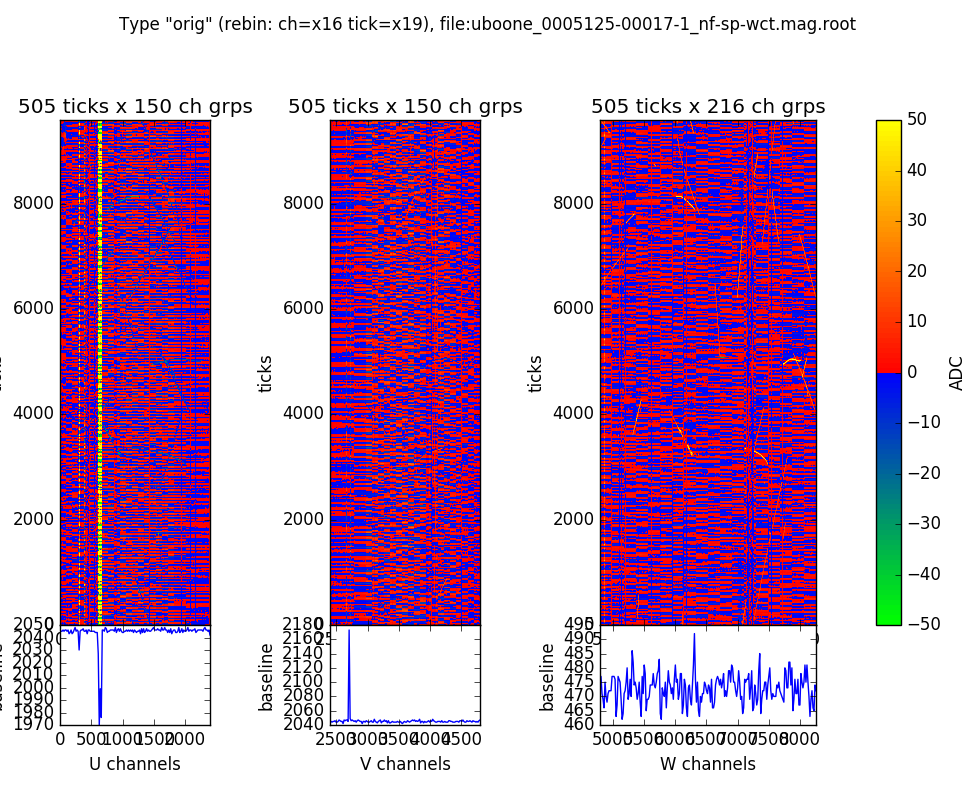
\includegraphics[width=5cm]{figures/uboone_0005125-00017-1_nf-sp-wct-orig_thumb.png}%  
  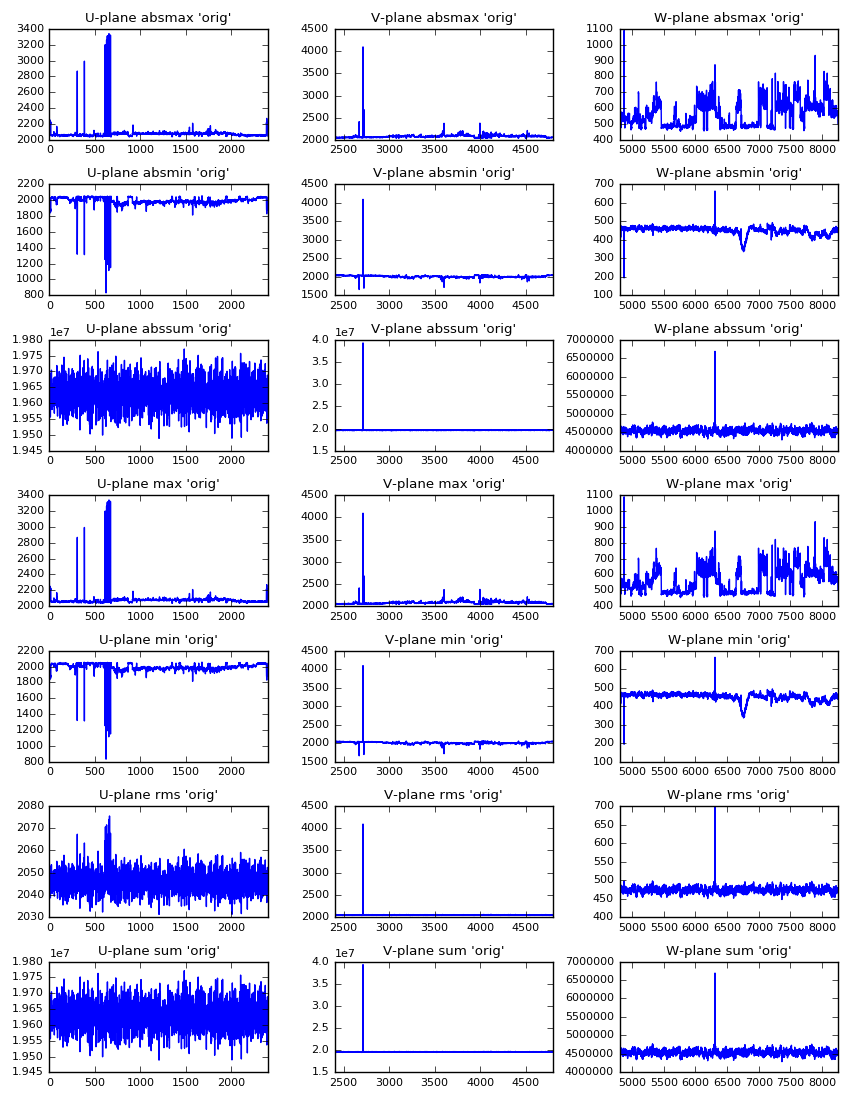
\includegraphics[width=5cm]{figures/uboone_0005125-00017-1_nf-sp-wct-orig_reduc.png}
\end{frame}

\begin{frame}[fragile]
  \frametitle{Noise Filtered ``raw''}
  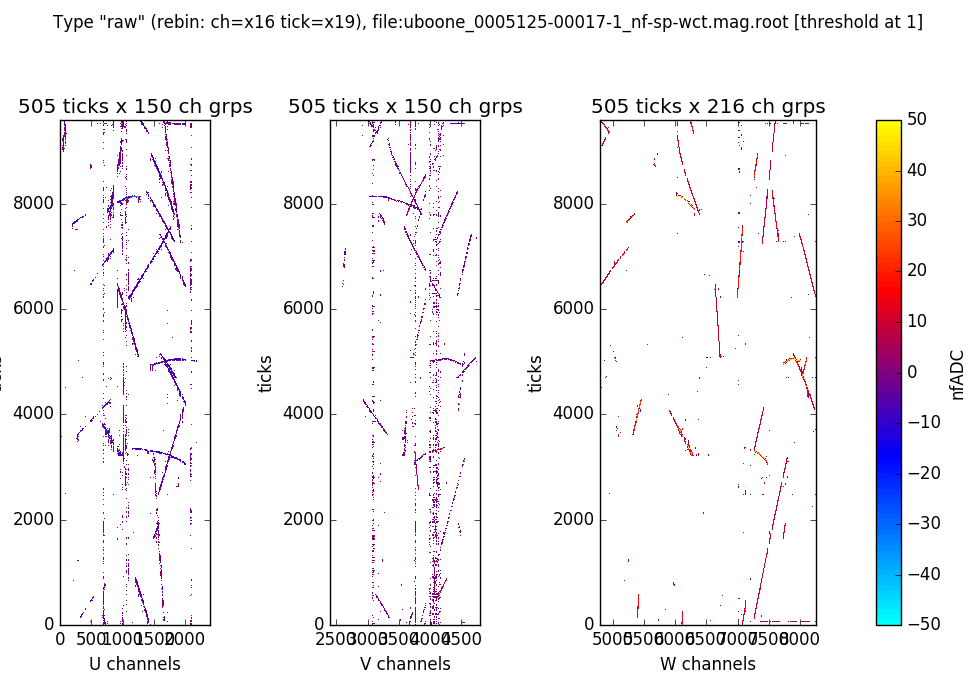
\includegraphics[width=5cm]{figures/uboone_0005125-00017-1_nf-sp-wct-raw_thumb.png}%  
  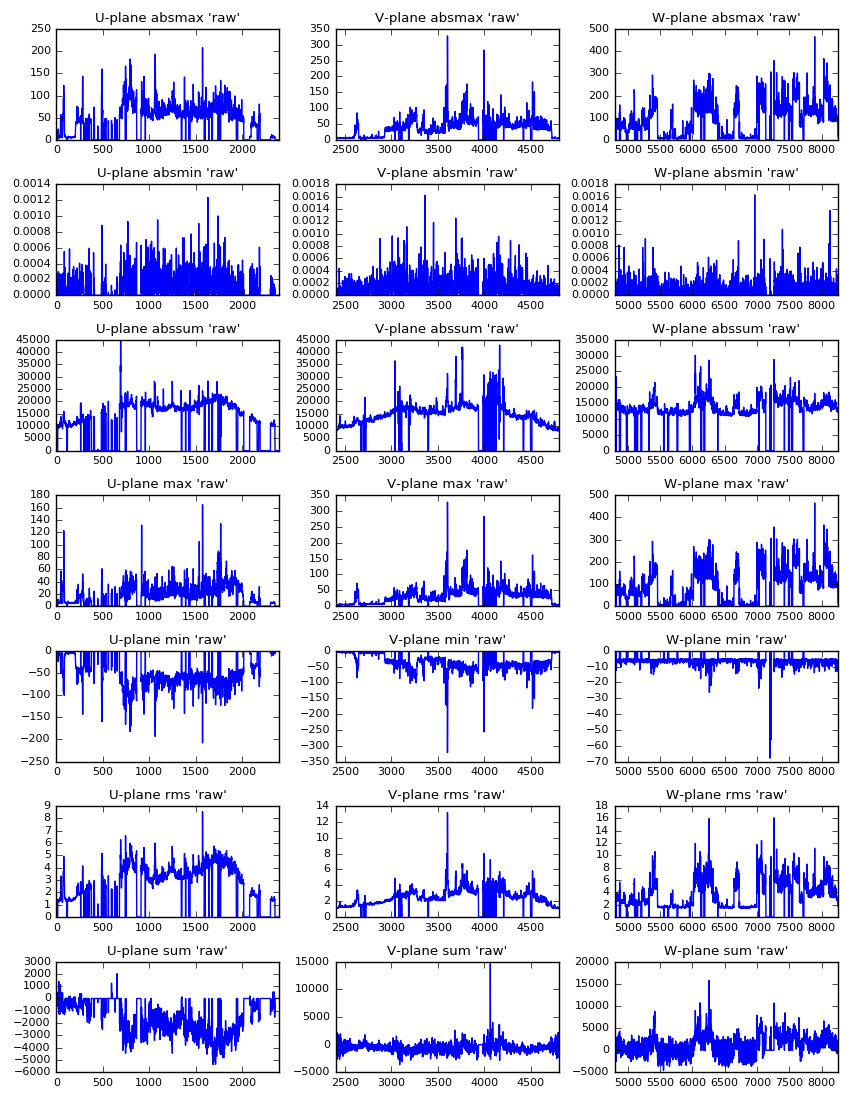
\includegraphics[width=5cm]{figures/uboone_0005125-00017-1_nf-sp-wct-raw_reduc.png}
\end{frame}

\begin{frame}[fragile]
  \frametitle{Signal Processed with Wiener Filter}
  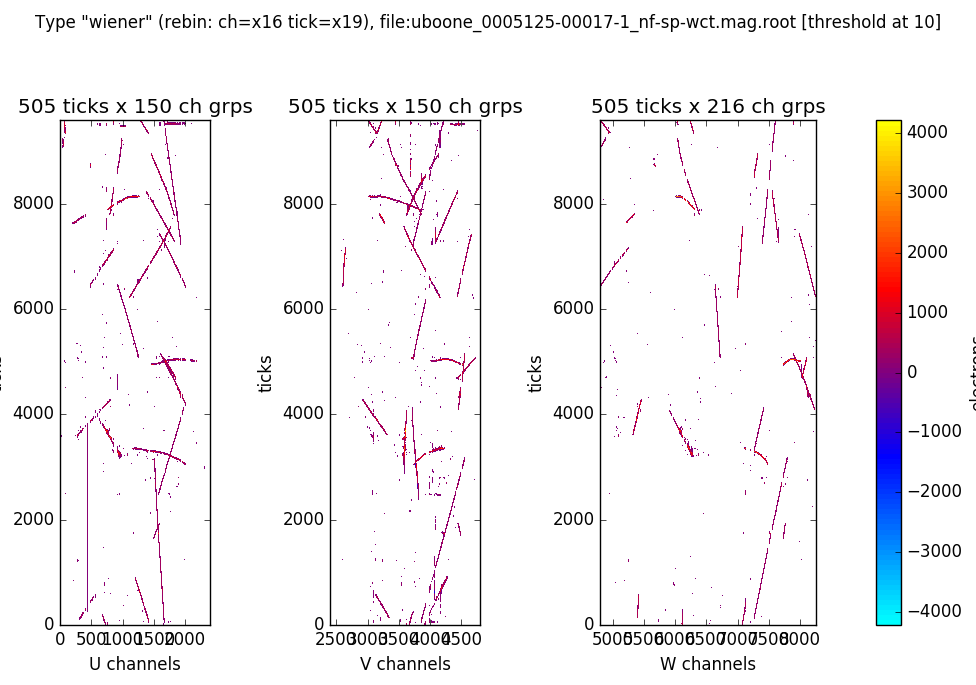
\includegraphics[width=5cm]{figures/uboone_0005125-00017-1_nf-sp-wct-wiener_thumb.png}%  
  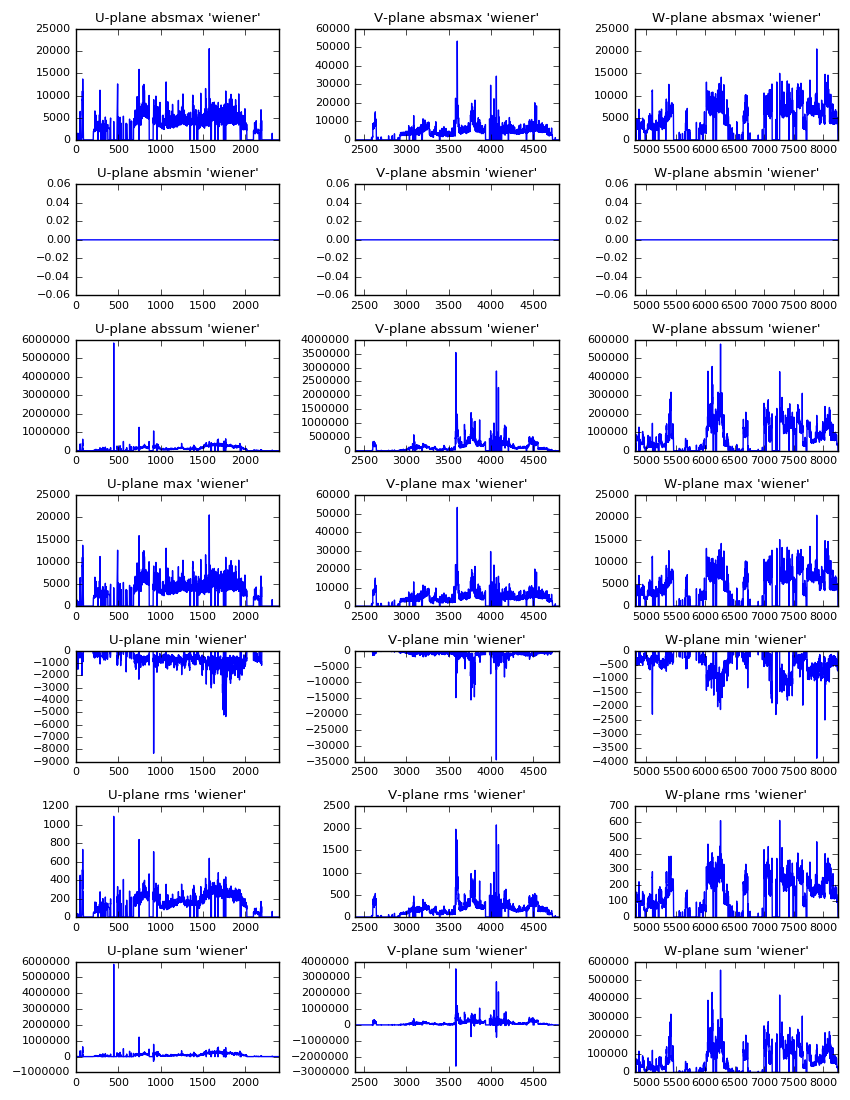
\includegraphics[width=5cm]{figures/uboone_0005125-00017-1_nf-sp-wct-wiener_reduc.png}
\end{frame}

\begin{frame}[fragile]
  \frametitle{Signal Processed with Gauss Filter}
  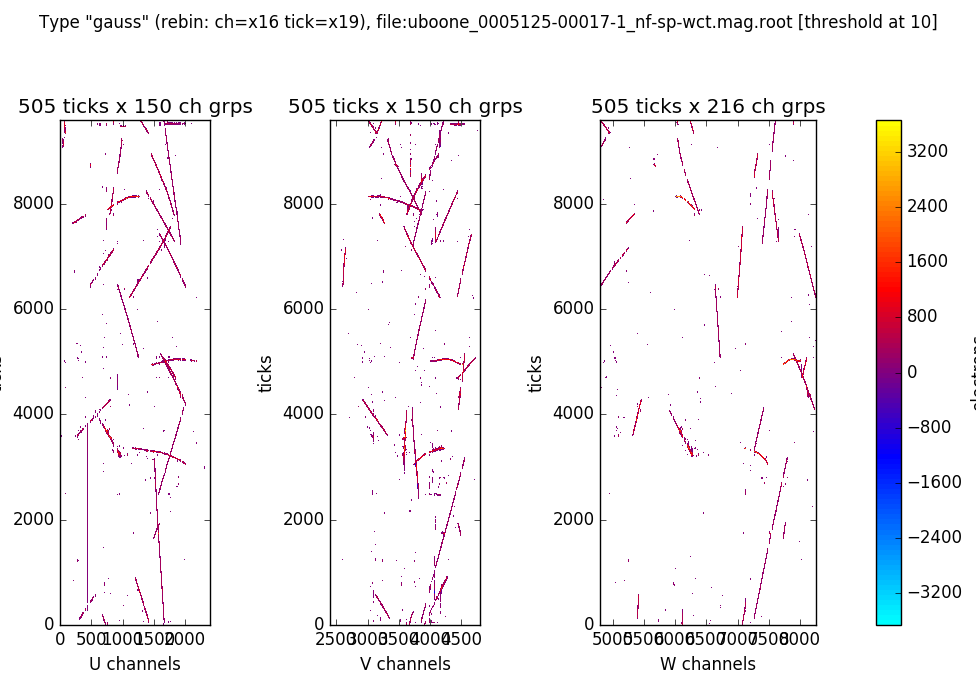
\includegraphics[width=5cm]{figures/uboone_0005125-00017-1_nf-sp-wct-gauss_thumb.png}%  
  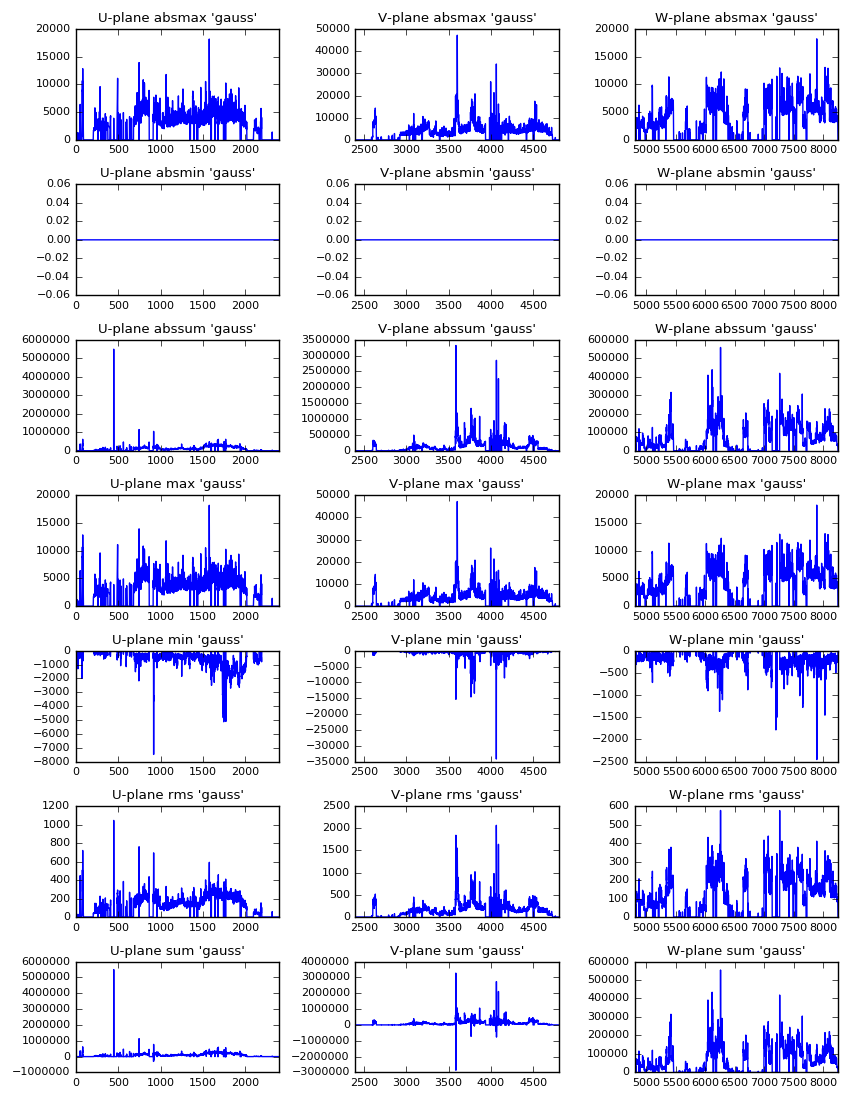
\includegraphics[width=5cm]{figures/uboone_0005125-00017-1_nf-sp-wct-gauss_reduc.png}
\end{frame}

\begin{frame}[fragile]
  \frametitle{Super Exciting WCT-WC/LS ``diffs''}
  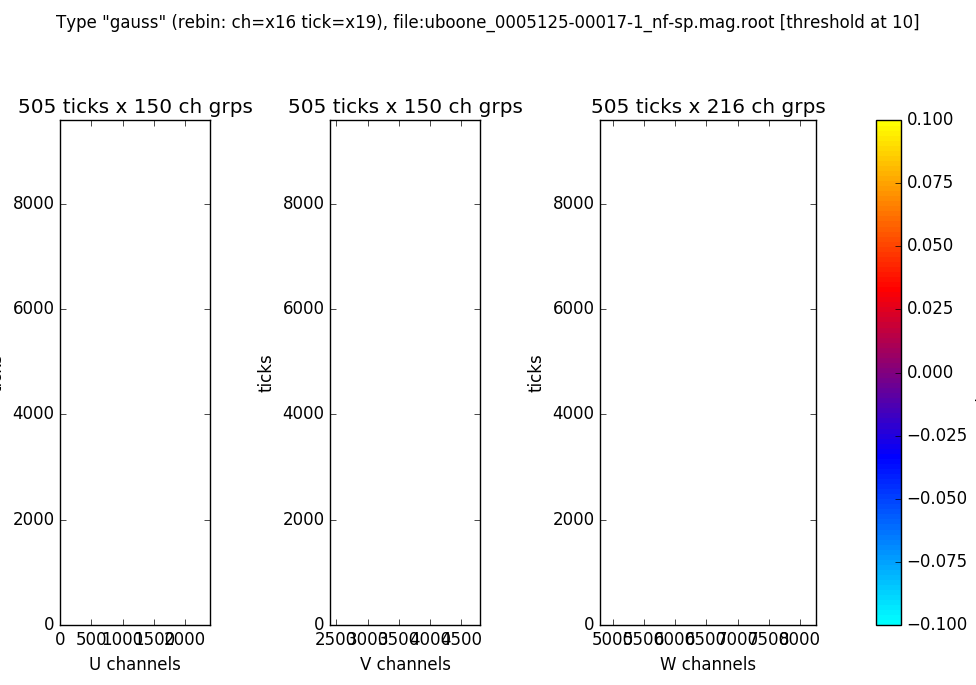
\includegraphics[width=5cm]{figures/uboone_0005125-00017-1_nf-sp-gauss_thumb.png}%  
  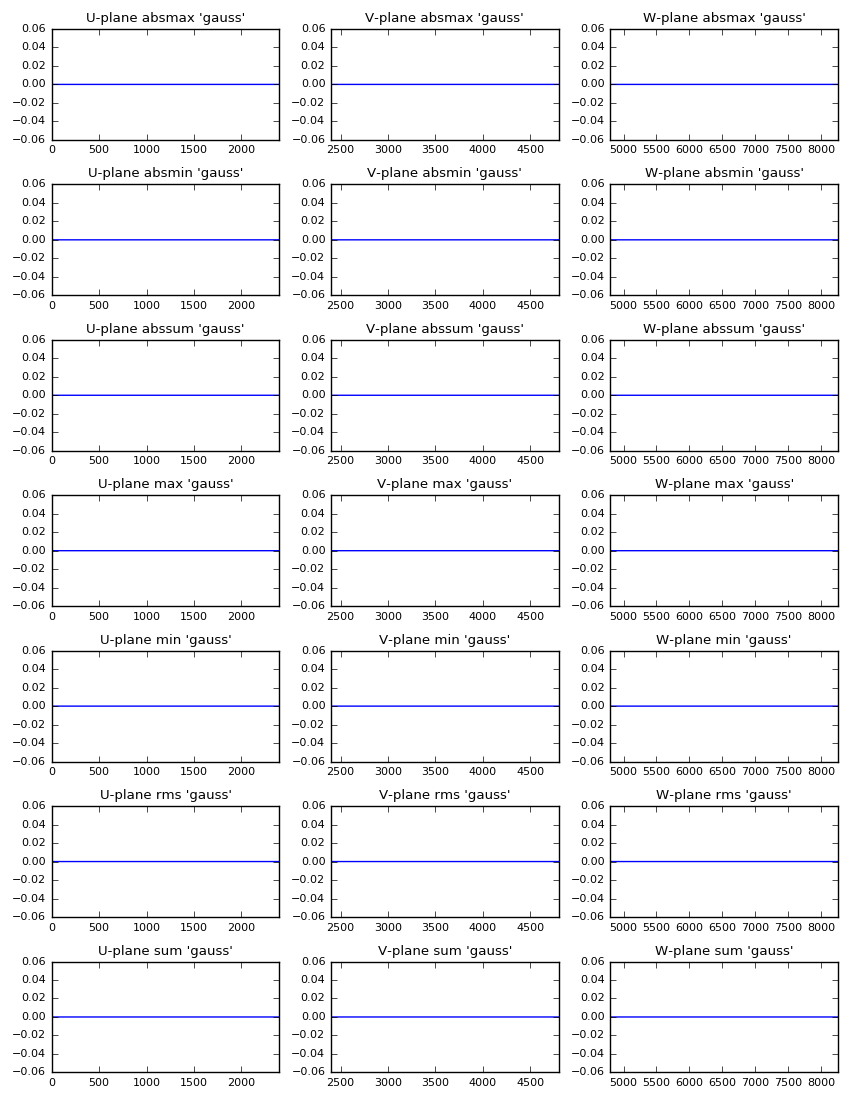
\includegraphics[width=5cm]{figures/uboone_0005125-00017-1_nf-sp-gauss_reduc.png}
\end{frame}


\section{Unsolicited Opinions}

\begin{frame}
  \frametitle{Unsolicited opinions on a uBoone CI}
  
  \begin{itemize}\footnotesize
  \item Provide a limited and \textbf{fixed input data} file set
    spanning all detector running.  MC can/should be run as a test itself.
  \item System must allow for \textbf{dependencies} between test jobs.  
    \begin{itemize}\scriptsize
    \item Test validity of intermediate output files.
    \end{itemize}
  \item  Allow tests in various languages/systems (not just art/C++).
  \item Allow various output files and post process them for validity.
  \item But, also make standardized JSON summary file for every test.
  \item \textbf{Integration tests likely dominate} over unit tests.
  \item Crucial to have \textbf{blessed output} which is automatically compared to output of each run.
    $\to$ Just as crucial to make it \textbf{easy to rebless}.
  \item Must have \textbf{fast notification} of failures to \textbf{responsible parties}.
  \item Failures must have \textbf{real repercusions} or they won't get addressed.
  \item Probably obvious: uBoone should try to exploit FNAL Jenkins.
  \item Likely \texttt{wire-cell-validate} will continue in its weird
    form but can be mined as a source of jobs for a ``real'' CI.
  \end{itemize}
\end{frame}

\end{document}


%%% Local Variables:
%%% mode: latex
%%% TeX-master: t
%%% End:
